\chapter{Memory Management}

In irreversible languages once it is determined that some data is no longer
needed it can simply be deleted and reallocated as needed.

In a reversible computation memory management is somewhat complicated by the
reversibility constraint since a bit cannot be simply set to zero and reused
when it is no longer needed.

Additionally working within the circuit model means that all planning of memory
allocation must be done at compile time.


\section{Janus}

Janus\cite{YG:2007,LD:1982} is a reversible programming
language.  It's main focus is not to be a circuit description language, but to
be logically reversible. As a result of logical reversibility it does have some
useful properties which help which compiling to circuits.

Janus guarantees that all programs implemented in it are reversible. Since each
statement in the language is reversible any ancilla used can be cleaned up in
between statements.

\subsection{Modification Operators}

Janus uses modification operators for operations that can be done in-place. For
example the addition modification operator, \verb|+=|. Operations that cannot be
done in place can only occur to the right of an in place operator. These
operations can then be implemented, the result can be applied in place to the
left hand side value, and then cleaned up using Bennett if necessary. This means
that memory need only be allocated temporarily for each modification statement.

\subsection{If Conditions}
If conditions require a pre-condition (used to choose which branch to take),
and a post-condition (true if and only if the top branch is taken).

These are very useful in the context of memory management. The pre-condition can
be used to set a bit which controls which operations are preformed. The
post-condition can be used to clear this bit as the pre-condition may no longer
be true after the loop is preformed.

\todo{add diagram}

\section{Pebble Games and Garbage Collection}

\subsection{Reversible Pebble Game}
Bennett\cite{Bennett:89} describes computations as a chain with the state of
each node computed from the node preceding it. This model allows memory
management using pebble games.

The rules of Bennett's reversible game are as follows:

\begin{enumerate}

  \item A pebble can be added to a node if and only if all predecessors of the
    node have pebbles

  \item A pebble can be removed from a node if and only if all predecessors of
    the node have pebbles

\end{enumerate}

The space complexity of the game is given by the maximum number of pebbles which
are in play at any given time. It has been shown that in general computing the
space complexity for an arbitrary DAG is PSPACE-complete \cite{chan13}.

Strategies for playing this games have been analyzed in the case of the one
dimensional directed graph, for example Knill \cite{knill:95} gives a time
optimal strategy for a given space bound.

\subsection{MDD}

Lacking in the original pebble game is an effective way to represent mutation.
For example addition via the mapping $(a,b) \mapsto (a,a+b)$ is a reversible
operation. In order for strategies from the reversible pebble game to be applied
to a circuit using this operation generically it would have to be made out of
place by copying the $b$ input and thus losing the advantages that may have been
gained by using an in-place operation.

In order to better represent in-place operations a new pebble game is proposed.
Rules one and two are similar to the reversible pebble game. The third rule
which requires labeled edges of two types has been added:

\begin{enumerate}

   \item A new pebble can be added to a node if and only if all predecessors of
     the node have pebbles.

   \item A pebble can be removed from a node if and only if all predecessors of
     the node have pebbles.

   \item A pebble may be moved forward or backward along a mutation edge if all
     predecessors of the destination node have pebbles.

\end{enumerate}

Note that since using the move described in the third rule is optional any
strategy that can be used in the reversible pebble game is a valid strategy
here. We also inherit the PSPACE-completeness (\cite{chan13}) of solving the
Reversible Bennett game since any graph which does not include mutation edges is
played by the rules of the reversible pebble game.

\subsection{Converting a Computation to an MDD}

\paragraph{Nodes} represent a register in some state.

\paragraph{Mutation Edges} represent operations which transform the value
of a register. The parent and child node of an edge represent the state of the
register before and after (respectively) the computation. Each node may have
only a single input and output mutation edge. A chain of nodes connected by
mutation edges represents all computations which change the contents of a
register.

\paragraph{Dependency Edges} represent values upon which a computation
depends. In order for a computation defined by a mutation edge to be implemented
all parent nodes along dependency edges pointing to the child node of the
mutation edge must be available.

For example the computation $(a,b)\mapsto(a,a+b)$ might be represented as a
solid arrow from the node $b$ to the node $a+b$ with a dependency arrow coming
from $a$.


\subsection{Computing the Cost of a Strategy}

In order to compute the cost of a given strategy when it is applied a few
new rules are needed:

\begin{enumerate}
    \setcounter{enumi}{3}
  \item Each node has a computation cost which is payed when placing a new pebble on
    it or sliding an existing pebble to it.
  \item Each node has a space cost which gives the contribution of that node to
    the overall space complexity when it is pebbled.
\end{enumerate}

The goal of this game is to come up with a set of moves the minimizes the total
movement cost as well as the space complexity.

When implementing the graph as a circuit we may preform the computations in any
valid topological ordering. Further if there are multiple computations which
could be next in a given ordering they can be preformed in parallel.

\subsection{Eager Cleanup}

When using the Revs ``eager cleanup'' method data dependencies are tracked in
order to minimize the time that intermediate values are kept allocated.

If a value is no longer needed in a computation it can then be checked that the
information needed to clean it up is available. If so it can immediately be
cleaned and the ancilla can be freed for future use in the computation. To track
this a heap of currently available ancilla is kept.  This ensures that the
lowest available numbered ancilla is always the one allocated so ancilla use is
minimized.

Eager cleanup is possible when all dependencies are one-way.

\begin{marginfigure}
  \includegraphics[width=0.8\hsize]{images/oneway.pdf}
  \caption{One Way}
\end{marginfigure}

\begin{marginfigure}
  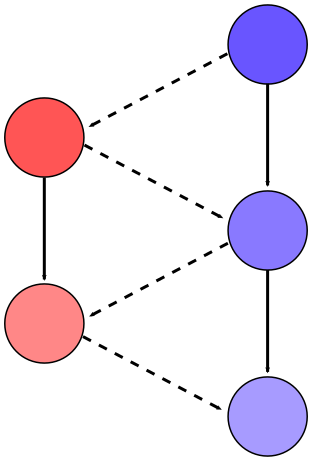
\includegraphics[width=0.8\hsize]{images/interdependent.pdf}
  \caption{Interdependent}
  \label{fig:interdep}
\end{marginfigure}

\todo{Rewrite this in terms of the game}
\begin{theorem}

Let $G=(V,E)$ be an MDD that is obtained from a given irreversible program
${\mathcal P}$.  Assume that all mutation paths in $G$ are pairwise one-way
dependent.  Then the circuit ${\mathcal C}$ produced by the \textsc{Eager}
cleanup method in Algorithm \ref{alg:eager} is correct in the sense that it
computes the same function as the original program ${\mathcal P}$ for some
assignment of the input values, ${\mathcal C}$ is reversible, and all ancillas
that may be used by ${\mathcal C}$ are returned in their initial state at the
end of the computation.

\end{theorem}

\begin{proof}

It is clear that the circuit computed by ${\mathcal C}$ is reversible as it uses
only reversible gates in its composition.  Furthermore, by construction, it
computes the given function on some of the output wires.  It remains to show
that all ancilla used during the computation, and inputs which have mutation
paths in the MDD G, can be cleaned up, i.e., can be returned to the initial
state.

Our proof is by induction on the number $k$ of mutation paths $P_1, \ldots, P_k$
inside the MDD $G$. The base case is trivial as if $k=1$ there is only one
mutation path and clearly this path either leads to an output, in which case no
cleanup is necessary, or leads to a node that has to be cleaned up. However,
since all inputs to the path are still available by assumption, the output of
the path, i.e., its last node, can simply be moved backward step by step,
uncomputing each intermediate result, until the initial state is recovered.

We strengthen out inductive hypothesis slightly by assuming that we can return
the final state of each path $P_1, \ldots, P_k$ to an arbitrary intermediate
state. Intuitively, we think of the state ``sliding up and down the mutation
path''. Now, we make the inductive step to $k+1$ paths. Recall that a node $v$
can be reversed if all their dependency edges pointing to $v$ are available
nodes, i.e., nodes which we can compute from the available data, by sliding the
final output either up or down the mutation path. If all dependency arrows of a
path point to available nodes, that segment of the path can be reversed. We
hence can make the inductive step as follows: Assume that the paths $P_1,
\ldots, P_{k+1}$ are arranged in topological order. Let the $v$ be the node
holding the current state of the last path $P_{k+1}$, i.e., by assumption on the
one-wayness of the graph, all edges point into $P_{k+1}$ and none points
backward. Now, consider all nodes in $P_1, \ldots, P_k$ that would have to be
available in order to move $v$ one step backward. By induction, we can slide the
states for each path into the location that is needed to make this information
available for $v$ to move backward one step. Repeating this argument, we see
that we can move the state anywhere along the last path $P_{k+1}$ thereby
showing that cleanup is possible and algorithm \textsc{Eager} will find this
cleanup strategy.

\end{proof}

\subsection{Triangles and Incremental Cleanup}
\Cref{fig:interdep} shows a graph where eager cleanup fails. The red mutation
path depends on previous values of the blue path in order to be cleaned.

\subsection{Circuit Generation}
Circuit generation is defined by creating a generation function for each
type of move allowed in the game then using that set of functions to convert a
graph and move set into a circuit.

We start with a circuit consisting of registers corresponding to the input nodes
of the graph.

\begin{itemize}
    \item Place Pebble:
    \item Remove Pebble:
    \item Slide Pebble:
\end{itemize}
